\section{Research Methodology}

\subsection{SLR Methodology Planning Protocol}
% 3 section our plan to answer the four mentioned questions 
In order to address the first research question(\textbf{RQ1}), a systematic literature review will be carried out in this paper. During the systematic literature review the main theme is to identify the security schemes presented in the literature to ensure the authentication of data flow between the virtual world(DT) and the physical object(sensors). Under subcategory of this main question, the concept of Digital Twin will be also studied and analysed. In this section, we briefly describe the planning protocol methodology for conducting systematic literature review as follow. 

Based on the first research question(\textbf{RQ1}), we identify 5 key terms that we plan to use for retrieving research articles from research databases, these are "Digital Twin", "IoT" "Authentication", "Security", and "communication". The first three key terms are most important keywords and SHOULD be included together in the paper. where as, the last two key terms are not mandatory to be present in the paper. The main key terms and their accepted variants are outline in Table \ref{keyterms}. 

\begin{table}[!ht]
    \centering
    \begin{tabular}{|l|l|}
    \hline
        \textbf{Key terms} & \textbf{Varients / Synonyms / Similar Semantic Meaning} \\ \hline
        Digital Twin & DT, Digital-Twin, Digital-Twins, Twins, Digitalization, Virtual Clone \\ \hline
        Internet of Things & IoT, Sensors, Actuators,  \\ \hline
        Authentication & Certificate, Verification\\ \hline
        Security & Integrity, Confidentiality, Cybersecurity,  \\ \hline
        Communication & Channel, message, messages \\ \hline
    \end{tabular}
    \caption{Main Keyterms }
    \label{keyterms}
\end{table}

As a base for searching relevant literature we use of well know computer science archives: IEEE Xplore according to \cite{kofod-petersen_how_nodate} and Scopus. In this systematic literature review part of the project, we only focus on articles published between 20016 and 2022 (7 years). The reason we choose those date is, according to systematic literature conducted by Kukushkin et al. \cite{kukushkin_digital_2022}, majority Digital Twin related articles are published in the last seven years.
\\
The following table shows few offline and online tools we used in for the systematic literature review. 
\begin{table}[!ht]
    \centering
    \begin{tabular}{|l|l|}
    \hline
        \textbf{Name of Tools} & \textbf{Purse / Function} \\ \hline
        Excel & To remove duplication, get insight \\ \hline
        VOSviewer & Bibliometric analysis \\ \hline
        Researchrabbit & For validating VOSviewer map,  \\ \hline
        Connectedpapers & For validating VOSviewer map,  \\ \hline
        parsifal & To document the whole systematic literature review process \\ \hline
    \end{tabular}
    \caption{Tools used for SLR  }
    \label{slrtools}
\end{table}

\subsection{Implementation Methodology}
To address research question three(\textbf{RQ3)}, we will implement our proposed authentication scheme on an open-source Digital Twin platform called Ditto and on one of microcontroller manufactured by Pycom called ESP32. The authentication scheme is based on a lightweight cryptographic algorithm standardized by NIST on March 2021.Ditto is an open source framework developed and maintained by Eclipse Foundation to facilitate the interaction between Digital Twin and IoT devices\cite{noauthor_eclipse_nodate}. We opt to ESP32 chipset because it can be programmed with micropython which is an implementation of Python3 for microcontroller. 
To answer our last research question, we will test our implementation using a power measuring tool to estimate the performance of the proposed schemes in terms of power consumption, execution time, and storage complexity.

% \begin{figure}[H]
%     \centering
%     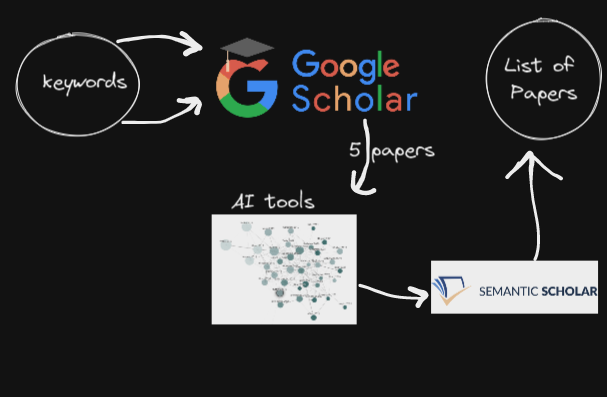
\includegraphics[width=1\textwidth]{images/method.png}
%     \caption{Research Methodology}
%     \label{fig:method}
% \end{figure}

% \subsection{Literature review methodology}
% Focus area of literatur review 
% Database used for paper extraction 
% Search keyword used
% Fiiltering mechanism 
% The tools we use to select papers. parameters used as factor of selection 

% \subsection{Problem solution methodology}